% CONSIDERAÇÕES FINAIS--------------------------------------------------------------------

\chapter{Considerações Finais}
\label{chap:consideracoesFinais}

A experiência de estágio no TRE-PB adicionou propriedade aos conhecimentos adquiridos ao longo da jornada como aluno e desenvolvedor de sistemas para internet. Atuar em diferentes papéis durante as fases do projeto ajudou a fixar conceitos e valorizar a importância de um bom planejamento para conclusão de um projeto de sucesso. 

A especificação de requisitos através da análise das histórias de usuário, nem sempre aconteceu de maneira natural, muitas vezes foi necessário capturar mensagens implicitas nos relatos do cliente e até mesmo investigar seu ambiente de trabalho. Documentar as funcionalidades necessárias para a estimativa e o desenvolvimento do sistema foi um trabalho que envolveu todo o time.
Codificar os mais variados requisitos utilizando diversos conceitos de programação orientada a objetos, bem como tecnologias como Spring e JSF, mais uma vez mostrou a importância de ter um time em total sincronia, pois divervas funcionalidades estão diretamente ligadas umas as outras. Receber feedbacks com sugestões ou críticas em relação a uma funcionalidade que foi implementada ajudou a pensar no desenvolvimento de novas ou na refatoração.

O sistema passou a ser utilizado em sua plenitude a partir de agosto de 2017 e em 2018 terminou o ano sendo o 4º sistema mais usado em todo o TRE com 23.375 transações conforme \autoref{fig:figura-ranking2018}. Já em 2019, até março, foram registradas 4.006 transações, já sendo o 3º sistema mais utilizado.

\begin{figure}[!htb]
    \centering
    \caption{Veículos - Ranking 2018}
    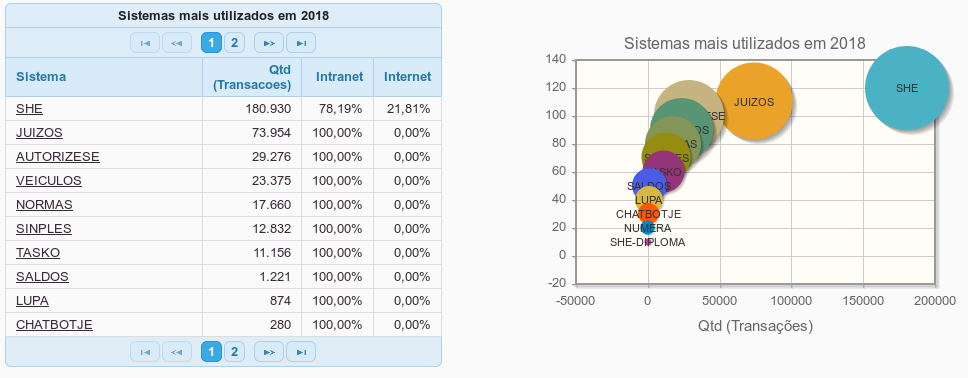
\includegraphics[width=0.75\textwidth]{./dados/figuras/ranking2018.png}
    \fonte{SEDES}
    \label{fig:figura-ranking2018}
\end{figure}

Novas funcionalidades já estão previstas e cadastradas como demandas que serão desenvolvidas. Uma delas é a automatização do processo de captura da quilometragem e da rota percorrida pelo motorista, que através de um equipamento de GPS deverá trasmirir os dados diretamente para a aplicação. Outras demandas surgiram com o uso da aplicação, dentre algumas que são correções de \textit{bug}, surgem outras que são classificadas como melhorias e foram sugeridas pelos usuários. Atualmente está em desenvolvimento a versão 1.3.0 e dentre outras melhorias e correções, está sendo implementado uma funcionalidade que notifica o gestor de forma sonora e visual quando uma nova solicitação de viagem é cadastrada. A necessidade dessa funcionalidade, surgiu no período das eleições de 2018, onde o gestor do sistema passou a receber um número mais elevado de solicitações que precisavam ser analisadas mais rapidamente.

A possibilidade de mensurar a quantidade de viagens realizadas pela frota do Tribunal e a quilometragem percorrida pelos veículos, distribuir motoristas de forma mais equilibrada, verificar a disponibilidade de motoristas ou veículos, ajustar passageiros em rotas equivalentes, sem dúvidas, tem ajudado os gestores a estimar custos, diminuir e evitar despesas e tem facilitado o envio de relatórios com esses dados para os processos de auditorias que são realizados com frequência.